% presentaciones/sesion02-cap02/sesion02.tex
% Sesión 2 — Capítulo 2: Perfil, segmentación y mercado meta digital
% Laboratorio: Gestión de datos, comportamiento y perfiles del consumidor digital
% Lic. en Mercadotecnia Digital · ESCA Unidad Santo Tomás · IPN
% Fuente de contenido: libro-consumidor-digital/partes/parte1/cap02.tex
% Figuras reutilizadas del libro (TikZ y MATLAB) sin copiarlas: ver \graphicspath y \input.
\documentclass[aspectratio=169,xcolor=dvipsnames]{beamer}
\usetheme{Berlin}

%----------------------------------------------------------------------------------------
%   PALETA INSTITUCIONAL IPN (Manual de Identidad Gráfica, Pantone 222C)
%----------------------------------------------------------------------------------------
\usepackage[dvipsnames,svgnames,x11names]{xcolor}
\definecolor{IPNguinda}{HTML}{6F1D46}       % Pantone 222C oficial — color primario
\definecolor{IPNguindaOsc}{HTML}{45102C}    % sombra / paleta secundaria
\definecolor{IPNguindaClara}{HTML}{F4E9EF}  % fondo de bloques normales
\definecolor{IPNdorado}{HTML}{B8975A}       % dorado — SOLO enlaces y detalles del cierre
\definecolor{IPNterracota}{HTML}{9C5B44}    % alertblock
\definecolor{IPNterracotaClara}{HTML}{F6ECE6}
\definecolor{IPNbronce}{HTML}{8C6B3F}       % exampleblock
\definecolor{IPNbronceClaro}{HTML}{F5F0E3}
\definecolor{IPNgris}{HTML}{58595B}         % texto secundario / notas

% Alias con los nombres de config/colores.tex del libro, para que las figuras
% TikZ del libro se puedan \input sin modificarlas
\colorlet{guindaIPN}{IPNguinda}
\colorlet{guindaIPNOsc}{IPNguindaOsc}
\colorlet{guindaIPNClara}{IPNguindaClara}
\colorlet{doradoIPN}{IPNdorado}
\colorlet{bronceIPN}{IPNbronce}
\colorlet{bronceIPNClaro}{IPNbronceClaro}
\colorlet{grisIPN}{IPNgris}
\definecolor{colorLaboratorio}{HTML}{1B6E7A}

\setbeamercolor{palette primary}{bg=IPNguinda,fg=white}
\setbeamercolor{palette secondary}{bg=IPNguindaOsc,fg=white}
\setbeamercolor{palette tertiary}{bg=IPNguindaOsc,fg=white}
\setbeamercolor{palette quaternary}{bg=IPNguinda,fg=white}
\setbeamercolor{structure}{fg=IPNguinda}
\setbeamercolor{title}{bg=IPNguinda,fg=white}
\setbeamercolor{frametitle}{bg=IPNguinda,fg=white}
\setbeamercolor{block title}{bg=IPNguinda,fg=white}
\setbeamercolor{block body}{bg=IPNguindaClara,fg=black}
\setbeamercolor{block title alerted}{bg=IPNterracota,fg=white}
\setbeamercolor{block body alerted}{bg=IPNterracotaClara,fg=black}
\setbeamercolor{block title example}{bg=IPNbronce,fg=white}
\setbeamercolor{block body example}{bg=IPNbronceClaro,fg=black}
\setbeamercolor{alerted text}{fg=IPNterracota}
\setbeamercolor{item}{fg=IPNguinda}
\setbeamercolor{section in toc}{fg=IPNguinda}
\setbeamercolor{footline}{bg=IPNguindaOsc,fg=white}

\usepackage[spanish,es-noshorthands,es-nodecimaldot]{babel}
\usepackage{csquotes}
\usepackage{hyperref}
\usepackage{graphicx}
\usepackage{booktabs}
\usepackage{array}
\usepackage{amsmath}
\setbeamertemplate{caption}[numbered]
\usepackage{xurl}
\usepackage{adjustbox}
\usepackage{tikz}
\usetikzlibrary{arrows.meta,positioning}
\usepackage{pgfplots}
\pgfplotsset{compat=1.18}

\graphicspath{{Figures/}{../../libro-consumidor-digital/figuras/matlab/}}
\newcommand{\figtikz}[1]{../../libro-consumidor-digital/figuras/tikz/#1}
\newcommand{\fuente}[1]{{\tiny\color{IPNgris}Fuente: #1}}

\hypersetup{
    colorlinks=true,
    linkcolor=IPNdorado,
    filecolor=IPNguinda,
    urlcolor=IPNguinda,
    citecolor=IPNguinda,
    pdftitle={Sesion 2 - Perfil, segmentacion y mercado meta digital},
    pdfauthor={Dr. Aboud Barsekh-Onji},
}

%----------------------------------------------------------------------------------------
%   CODE LISTINGS — sintaxis ESTÁNDAR del lenguaje
%----------------------------------------------------------------------------------------
\usepackage{listings}
\definecolor{backcolour}{rgb}{0.97,0.97,0.99}
\definecolor{codegreen}{rgb}{0,0.6,0}

\lstdefinestyle{MATLABStyle}{
  language=Matlab,
  basicstyle=\ttfamily\scriptsize,
  keywordstyle=\color{blue}\bfseries,
  commentstyle=\color{codegreen},
  stringstyle=\color{violet},
  breaklines=true,
  numbers=left,
  numbersep=5pt,
  frame=lines,
  backgroundcolor=\color{backcolour}
}
\lstset{style=MATLABStyle}

%----------------------------------------------------------------------------------------
%   TITLE CONFIGURATION
%----------------------------------------------------------------------------------------
\logo{
\includegraphics[height=0.75cm]{ipn-escudo.png}}
\title[Sesión 2 · Perfil y segmentación]{Perfil, segmentación y mercado meta digital}
\subtitle{Sesión 2 · Unidad I — Capítulo 2}
\author{Dr. Aboud Barsekh-Onji}
\institute[IPN]{
    Instituto Politécnico Nacional \\
    \small ESCA Unidad Santo Tomás · Lic. en Mercadotecnia Digital \\
    \footnotesize Laboratorio: Gestión de datos, comportamiento y perfiles del consumidor digital
}
\date{\today}

%----------------------------------------------------------------------------------------
%   AUTO AGENDA AT EACH SECTION
%----------------------------------------------------------------------------------------
\AtBeginSection[]{
  \begin{frame}{Agenda}
    \tableofcontents[currentsection]
  \end{frame}
}

\begin{document}

\begin{frame}
    \titlepage
    \vspace{-4pt}
    \begin{center}
        {\tiny\color{IPNgris} ORCID: \href{https://orcid.org/0009-0004-5440-8092}{0009-0004-5440-8092}}
    \end{center}
\end{frame}

%------------------------------------------------
\section{Encuadre}
%------------------------------------------------

\begin{frame}{Ficha de la sesión}
\begin{columns}[T]
  \column{0.52\textwidth}
  \begin{block}{Unidad I}
    \small Comportamiento, perfil y gestión de datos del consumidor digital
  \end{block}
  \begin{block}{Temas del programa (1.2 Perfil)}
    \scriptsize
    \begin{itemize}
      \item[1.2.1] Segmentación del mercado digital y variables
      \item[1.2.2] Mercado meta o \textit{target} digital
      \item[1.2.3] Tipos de perfil del consumidor digital
      \item[1.2.4] Radiografía del consumidor digital en México y el mundo
      \item[1.2.5] Diversidad de perfiles por modelo de negocio-industria
    \end{itemize}
  \end{block}
  \column{0.44\textwidth}
  \begin{block}{Carga horaria}
    \small Teoría 3.0 h · Práctica 2.0 h\\ Aprendizaje autónomo 1.0 h
  \end{block}
  \begin{exampleblock}{Competencia de la unidad}
    \small Identifica el comportamiento del consumidor digital y su evolución a partir de sus tipos de perfil y gestión de datos.
  \end{exampleblock}
\end{columns}
\end{frame}

\begin{frame}{Al terminar la sesión podrás\ldots}
\begin{enumerate}
  \item \textbf{Aplicar} el proceso segmentación-\textit{targeting}-posicionamiento (STP) a un caso de mercado digital.
  \vspace{6pt}
  \item \textbf{Distinguir} segmentación rígida de segmentación difusa y justificar cuándo cada una es preferible.
  \vspace{6pt}
  \item \textbf{Describir}, con datos verificados, la radiografía del consumidor digital mexicano frente al panorama internacional.
\end{enumerate}
\vspace{8pt}
\begin{alertblock}{Recordatorio}
  Actividad de investigación en biblioteca (Sesión 1): entrega a más tardar el \textbf{viernes 2 de octubre}, en su carpeta del portafolio.
\end{alertblock}
\end{frame}

\begin{frame}{Arranque: ¿quién eres para cada app?}
\begin{columns}[T]
  \column{0.55\textwidth}
  \begin{exampleblock}{Pregunta de arranque}
    Piensen en dos apps que usen a diario, por ejemplo una de \textbf{streaming} y la de su \textbf{banco}.\\[4pt]
    ¿Qué \enquote{tipo de usuario} creen que es cada una de ustedes para cada app? ¿Es la misma etiqueta?
  \end{exampleblock}
  \vspace{4pt}
  {\small\color{IPNgris} Puente con la Sesión 1: la doble naturaleza persona/dato.}
  \column{0.41\textwidth}
  \begin{block}{Dinámica (10 min)}
    \small
    \begin{enumerate}
      \item Individual: escriban dos etiquetas, una por app (2 min).
      \item Parejas: ¿qué dato usó cada app para \enquote{etiquetarlos}?
      \item Pizarrón: lista de datos por tipo de negocio. Vuelve en la sección de industria.
    \end{enumerate}
  \end{block}
\end{columns}
\end{frame}

%------------------------------------------------
\section[Apertura]{Caso de apertura}
%------------------------------------------------

\begin{frame}{Una persona, dos perfiles}
\begin{columns}[c]
  \column{0.48\textwidth}
  \begin{block}{Plataforma de streaming}
    \centering\enquote{usuario \textbf{ocasional} de fin de semana}
  \end{block}
  \column{0.48\textwidth}
  \begin{exampleblock}{App bancaria}
    \centering\enquote{usuario de \textbf{alto compromiso}}
  \end{exampleblock}
\end{columns}
\vspace{8pt}
\begin{itemize}
  \item No hay contradicción: son \textbf{dos negocios midiendo comportamientos distintos} sobre la misma persona.
  \item Error común de la segmentación de manual: tratar al consumidor como si tuviera \textbf{una sola identidad de compra} fija, válida para cualquier categoría.
\end{itemize}
\vspace{4pt}
\begin{alertblock}{La tesis de la sesión}
  El perfil de un consumidor digital es \textbf{específico del comportamiento que se mide}, y muchas veces ni siquiera es una etiqueta única dentro de la misma categoría.
\end{alertblock}
\end{frame}

%------------------------------------------------
\section[STP]{1.2.1--1.2.2 Segmentación y mercado meta}
%------------------------------------------------

\begin{frame}{El origen: Wendell R. Smith (1956)}
\begin{block}{Segmentación de mercado}
  Ver un mercado heterogéneo \enquote{como un número de mercados homogéneos más pequeños, en respuesta a preferencias de producto diferentes entre segmentos importantes del mercado}.
\end{block}
\begin{columns}[T]
  \column{0.48\textwidth}
  \begin{exampleblock}{Diferenciación de producto}
    \small Adaptar el \textbf{mercado} al producto (una oferta, mucha promoción).
  \end{exampleblock}
  \column{0.48\textwidth}
  \begin{block}{Segmentación}
    \small Adaptar el \textbf{producto} a subgrupos del mercado con preferencias distintas.
  \end{block}
\end{columns}
\vspace{2pt}
\fuente{Smith (1956), \textit{Journal of Marketing}, 21(1), 3--8.}
\end{frame}

\begin{frame}{El proceso STP}
\begin{center}
  \resizebox{0.9\linewidth}{!}{\input{\figtikz{cap02-stp}}}
\end{center}
\vspace{4pt}
\begin{itemize}
  \small
  \item Smith aporta la \textbf{base conceptual}; el STP es su \textbf{sistematización posterior} en los manuales de Kotler.
  \item Hoy: STP sigue vigente como \textbf{marco de decisión}; lo que cambió es el \textbf{método} para llenarlo.
\end{itemize}
\fuente{elaboración propia.}
\end{frame}

\begin{frame}{Las variables: de la encuesta al dato conductual}
\small
\begin{center}
\begin{tabular}{@{}>{\raggedright}p{2.3cm}>{\raggedright}p{4.4cm}>{\raggedright\arraybackslash}p{6.2cm}@{}}
\toprule
\textbf{Variable} & \textbf{Versión clásica} (encuesta/censo) & \textbf{Equivalente digital} (dato conductual) \\
\midrule
Geográfica & Región, ciudad declarada & Geolocalización del dispositivo, IP, zona de entrega \\
Demográfica & Edad, sexo, ingreso declarados & Edad/sexo inferidos por plataforma; nivel socioeconómico por compra \\
Psicográfica & Estilo de vida, valores (encuesta) & Intereses inferidos por interacción con contenido y cuentas seguidas \\
Conductual & Frecuencia de compra declarada & Frecuencia, recencia y monto, \textbf{registrados directamente} \\
\bottomrule
\end{tabular}
\end{center}
\fuente{elaboración propia con base en Smith (1956), Solomon (2017) y Hoyer et al. (2024).}
\end{frame}

\begin{frame}{La verdadera revolución: el costo relativo}
\begin{columns}[c]
  \column{0.5\textwidth}
  \begin{alertblock}{Distinta en grado, no en naturaleza}
    La segmentación digital \textbf{no inventó variables nuevas}.
  \end{alertblock}
  \begin{block}{Lo que sí cambió}
    La variable \textbf{conductual} —antes la más cara, porque dependía de que el consumidor recordara y declarara su conducta— es hoy la \textbf{más barata}: el sistema la registra solo.
  \end{block}
  \column{0.46\textwidth}
  \centering
  \begin{tikzpicture}[
      caja/.style={rectangle, rounded corners, thick,
                   minimum width=4.6cm, minimum height=1.2cm, align=center, font=\small},
      flecha/.style={-{Stealth[length=3mm]}, thick, draw=IPNdorado}
    ]
    \node[caja, draw=IPNgris, fill=IPNgris!10] (antes) at (0,1.6) {\textbf{Antes:} encuesta\\ \scriptsize el consumidor recuerda y declara};
    \node[caja, draw=IPNguinda, fill=IPNguindaClara] (hoy) at (0,-0.6) {\textbf{Hoy:} registro automático\\ \scriptsize clic, compra, sesión};
    \draw[flecha] (antes) -- node[right, font=\scriptsize, align=left] {de la más cara\\ a casi gratuita} (hoy);
  \end{tikzpicture}\\[2pt]
  {\scriptsize Variable \textbf{conductual}}
\end{columns}
\end{frame}

\begin{frame}{Mercado meta (\textit{target}) digital}
\small
\begin{block}{Definición}
  Elegir, de entre los segmentos identificados, aquel o aquellos hacia los que la organización dirige su \textbf{oferta} y su \textbf{comunicación}.
\end{block}
\begin{columns}[T]
  \column{0.48\textwidth}
  \begin{exampleblock}{En medios masivos}
    \small El mercado meta se \textbf{declara} en el plan de mercadotecnia.
  \end{exampleblock}
  \column{0.48\textwidth}
  \begin{exampleblock}{En plataformas digitales}
    \small Además se \textbf{configura}: audiencias personalizadas, públicos similares (\textit{lookalike}), exclusiones.
  \end{exampleblock}
\end{columns}
\vspace{4pt}
\begin{alertblock}{Consecuencia operativa}
  Elegir mal el mercado meta ya no es solo un error estratégico: es un \textbf{parámetro mal configurado} que desperdicia presupuesto en cuestión de horas.
\end{alertblock}
\end{frame}

%------------------------------------------------
\section[Perfiles]{1.2.3 Tipos de perfil}
%------------------------------------------------

\begin{frame}{¿Existe una tipología científica de perfiles?}
\begin{alertblock}{Búsqueda deliberada, resultado negativo}
  Se revisaron las ediciones recientes de Solomon y Russell (2023) y de Hoyer, MacInnis y Pieters (2024): \textbf{no hay} una tipología académica de \enquote{tipos de perfil del consumidor digital} con autoría y método rastreables.
\end{alertblock}
\begin{columns}[T]
  \column{0.48\textwidth}
  \begin{block}{Blogs de mercadotecnia}
    \small \enquote{el informado}, \enquote{el social}, \enquote{el impulsivo}\ldots\\ Sin aparato metodológico ni autoría.
  \end{block}
  \column{0.48\textwidth}
  \begin{exampleblock}{\textit{El Cubo NORISO} (2015)}
    \small Delgado Soriano et al.: \textbf{ocho perfiles} de personalidad del consumidor digital. Tipología \textbf{de autor}, de divulgación, no revisada por pares.
  \end{exampleblock}
\end{columns}
\vspace{2pt}
\begin{center}\small Mismo criterio que la Sesión 1 con \textit{Marketing X.0}: útil, pero con el estatus que le corresponde.\end{center}
\end{frame}

\begin{frame}{Lo que sí tiene respaldo: el método}
\begin{block}{No una tipología cerrada, sino cómo construirla}
  El \textbf{clustering} permite a cualquier organización construir \textbf{su propia} tipología de perfiles a partir de \textbf{datos propios}.
\end{block}
\begin{center}
  \resizebox{0.66\linewidth}{!}{\input{\figtikz{cap02-rigida-vs-difusa}}}
\end{center}
\fuente{elaboración propia.}
\end{frame}

\begin{frame}{Frontera: segmentación difusa}
\begin{columns}[T]
  \column{0.54\textwidth}
  \begin{block}{\textit{Fuzzy c-means} (Bezdek, 1981)}
    \small Sobre los conjuntos difusos de Zadeh (1965), sustituye la casilla única por un \textbf{grado de pertenencia}:
    \[
      u_{ik} \in [0,1], \qquad \sum_{k} u_{ik} = 1
    \]
    del consumidor $i$ a cada segmento $k$.
  \end{block}
  \column{0.42\textwidth}
  \begin{alertblock}{¿Quién es el caso particular?}
    \small La rígida (\textit{k-means}) es el \textbf{caso límite} en que toda la pertenencia se concentra en un solo segmento: $u_{ik}\in\{0,1\}$.\\[4pt]
    La difusa es la formulación \textbf{general}; no al revés.
  \end{alertblock}
\end{columns}
\vspace{6pt}
\begin{center}\small El laboratorio implementa ambas sobre los mismos datos: la diferencia se \textbf{observa}, no solo se declara.\end{center}
\end{frame}

%------------------------------------------------
\section[Radiografía]{1.2.4 Radiografía del consumidor digital}
%------------------------------------------------

\begin{frame}{Radiografía del consumidor digital mexicano (2024)}
\begin{columns}[c]
  \column{0.55\textwidth}
  \begin{tikzpicture}
    \begin{axis}[
        width=\linewidth, height=5cm,
        ybar, bar width=16pt, ymin=0, ymax=6.8,
        symbolic x coords={18--24,25--34,35--44,55--64,65+},
        xtick=data,
        xlabel={grupo de edad (años)}, ylabel={horas diarias de internet},
        label style={font=\scriptsize}, tick label style={font=\scriptsize},
        nodes near coords, nodes near coords style={font=\scriptsize},
        enlarge x limits=0.15,
        axis lines*=left, ymajorgrids, grid style={IPNgris!25},
      ]
      \addplot[fill=IPNguinda, draw=IPNguindaOsc] coordinates {(18--24,5.7) (25--34,5.6) (35--44,4.7) (55--64,3.2) (65+,3.0)};
    \end{axis}
  \end{tikzpicture}\\
  {\tiny\color{IPNgris}El grupo 45--54 no se incluye: no está entre los datos verificados del libro.}
  \column{0.41\textwidth}
  \begin{block}{Adopción de internet}
    \small
    \begin{tabular}{@{}lr@{}}
      Zona urbana & 86.9\,\% \\
      Zona rural & 68.5\,\% \\
      Adultos 65+ & 42.1\,\% \\
    \end{tabular}
  \end{block}
  \fuente{INEGI, ENDUTIH 2024, Reporte de Resultados 9/25 y Comunicado 57/25.}
\end{columns}
\end{frame}

\begin{frame}{Lo que muestra la radiografía}
\begin{block}{1. La edad explica más que cualquier tipología}
  \small Relación casi \textbf{monótona}: a menor edad, más horas de conexión, con caída sostenida a partir de los 35 años.
\end{block}
\begin{block}{2. La brecha urbano-rural: 18.4 puntos}
  \small La segunda variable con mayor poder explicativo verificado en este capítulo.
\end{block}
\begin{alertblock}{Riesgo de sobreajuste}
  \small Saltar directo a variables psicográficas \enquote{vistosas} sin controlar edad y zona es construir categorías elegantes sobre una base demográfica que \textbf{ya explica buena parte de la varianza}.
\end{alertblock}
\end{frame}

%------------------------------------------------
\section[Industria]{1.2.5 Perfiles por modelo de negocio}
%------------------------------------------------

\begin{frame}{Cada negocio mide una variable de éxito distinta}
\small
\begin{center}
\begin{tabular}{@{}lll@{}}
\toprule
\textbf{Modelo de negocio} & \textbf{Optimiza por\ldots} & \textbf{Perfil resultante} \\
\midrule
Comercio electrónico & conversión y ticket promedio & comprador \\
Red social & tiempo de permanencia e interacción & audiencia \\
Fintech & frecuencia de uso y profundidad de producto & usuario financiero \\
\bottomrule
\end{tabular}
\end{center}
\begin{alertblock}{No existe un \enquote{perfil digital} único y portable}
  El perfil es una \textbf{función del negocio que lo construye}, no un atributo fijo de la persona.
\end{alertblock}
{\small\color{IPNgris} Retomen el pizarrón del arranque: ¿qué dato usaba cada app?}\\
\fuente{elaboración propia con base en el enfoque por mecanismos de Sheth y Jain (2026).}
\end{frame}

\begin{frame}{Regreso a la doble naturaleza (Sesión 1)}
\begin{center}
  \resizebox{0.72\linewidth}{!}{\input{\figtikz{cap01-doble-naturaleza}}}
\end{center}
\begin{itemize}
  \small
  \item El capítulo 2 la vuelve \textbf{operativa}: cuantos más negocios observan al mismo consumidor, más perfiles distintos y parciales de esa persona existen.
  \item \textbf{Ninguno de ellos está completo.}
\end{itemize}
\end{frame}

%------------------------------------------------
\section[Laboratorio]{Laboratorio MATLAB}
%------------------------------------------------

\begin{frame}{Laboratorio: segmentación rígida y difusa}
\begin{block}{Objetivo}
  Comparar \textit{k-means} contra \textit{fuzzy c-means} sobre datos \textbf{sintéticos} de consumidores e identificar qué proporción queda mal representada por una asignación única de segmento.
\end{block}
\begin{equation}
  J_m = \sum_{i=1}^{n}\sum_{k=1}^{c} u_{ik}^{m}\, \lVert x_i - v_k \rVert^2,
  \qquad \text{sujeto a } \sum_{k=1}^{c} u_{ik} = 1 \ \ \forall i
\end{equation}
\begin{itemize}
  \small
  \item $x_i$: vector de comportamiento del consumidor $i$; \ $v_k$: centro del segmento $k$.
  \item $u_{ik}\in[0,1]$: grado de pertenencia; \ $m$: exponente difuso ($m>1$; el script usa $m=2$, fijo).
\end{itemize}
\fuente{Bezdek (1981).}
\end{frame}

\begin{frame}{¿Cómo se evalúa cada segmentación?}
\begin{columns}[T]
  \column{0.48\textwidth}
  \begin{block}{Rígida: coeficiente de silueta}
    \small Compara la distancia de cada punto a su propio segmento contra la distancia al segmento más cercano.
    \vspace{4pt}

    Rango $[-1,1]$: cerca de 1, segmentos bien separados; cerca de 0 o negativo, traslapados.
  \end{block}
  \column{0.48\textwidth}
  \begin{exampleblock}{Difusa: pertenencia ambigua}
    \small Proporción de consumidores cuya pertenencia máxima \textbf{no supera 0.6}.
    \vspace{4pt}

    Cuantifica cuántos casos la segmentación rígida está \textbf{forzando} a una casilla que no les queda.
  \end{exampleblock}
\end{columns}
\end{frame}

\begin{frame}[fragile]{El script: \texttt{cap02\_segmentacion.m}}
\begin{columns}[T]
  \column{0.58\textwidth}
\begin{lstlisting}[basicstyle=\ttfamily\scriptsize]
%% ==================================
%  PARAMETROS: UNICA SECCION QUE
%  EL ESTUDIANTE DEBE EDITAR
%  ==================================
% [frecuencia, ticket (MXN), engagement]
centrosTipicos = [
    1.5,  350,  25    % "ocasional"
    4.0,  900,  78    % "leal"
    2.6,  600,  52 ]; % "intermedio"
dispersionTipica = [ ... ];  % misma forma
nClientesPorSegmento = 80;  % por arquetipo
\end{lstlisting}
  \column{0.38\textwidth}
  \begin{block}{Reglas y rangos}
    \scriptsize
    \begin{itemize}
      \item Cada \textbf{fila} es un arquetipo; $k$ = número de filas ($k\geq 2$).
      \item Frecuencia mensual, ticket en MXN, engagement 0--100.
      \item Datos \textbf{sintéticos} (\texttt{rng(42)}); el resto del script se ajusta solo.
    \end{itemize}
  \end{block}
  \begin{exampleblock}{Sin MATLAB}
    \scriptsize \texttt{cap02\_segmentacion\_\allowbreak interactivo.html}: mismos parámetros, casos A, B, C y \enquote{Agregar arquetipo}.
  \end{exampleblock}
\end{columns}
\end{frame}

\begin{frame}{Salida con los arquetipos por defecto}
\begin{center}
  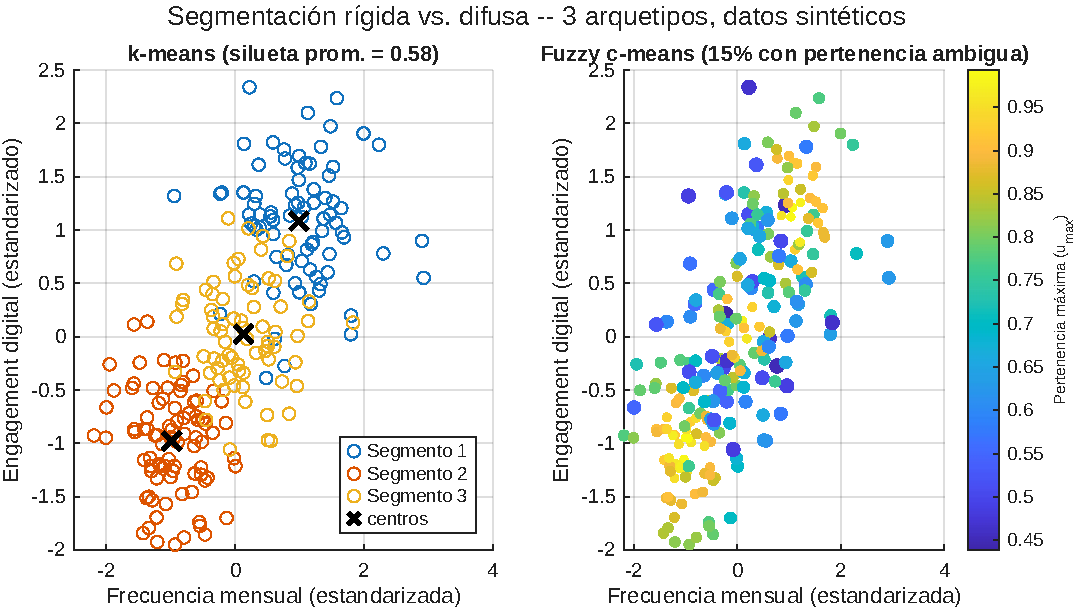
\includegraphics[width=\linewidth,height=0.56\textheight,keepaspectratio]{cap02_segmentacion_comparacion.pdf}
\end{center}
\vspace{-4pt}
\begin{center}
  \small \textit{k-means}: silueta promedio \textbf{0.58} \quad · \quad \textit{fuzzy c-means}: \textbf{15\,\%} de consumidores sin pertenencia dominante
\end{center}
\fuente{elaboración propia, MATLAB, datos sintéticos, \texttt{rng(42)}.}
\end{frame}

\begin{frame}{Interpretación de negocio}
\begin{columns}[c]
  \column{0.44\textwidth}
  \centering
  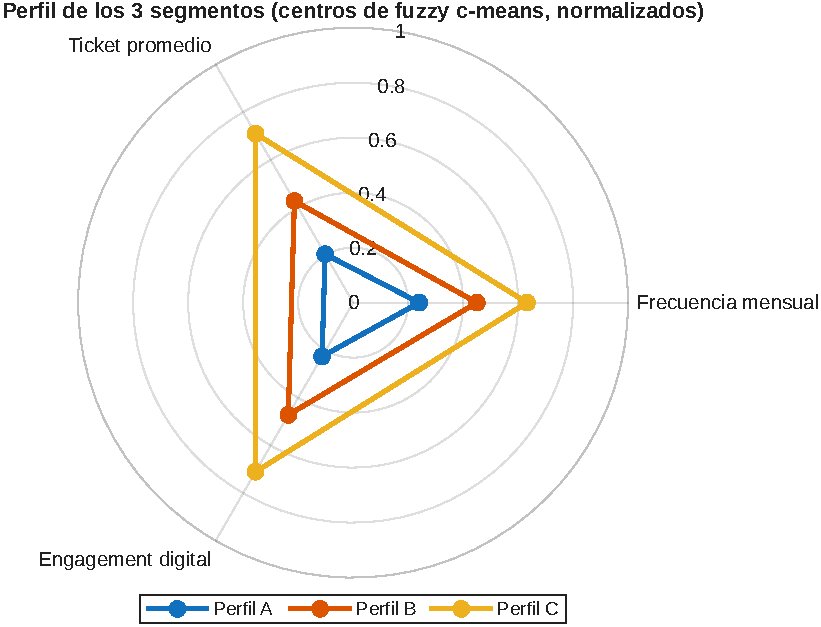
\includegraphics[width=\linewidth,height=0.66\textheight,keepaspectratio]{cap02_perfiles_radar.pdf}\\
  {\scriptsize Perfil de los segmentos (FCM, centros normalizados)}
  \column{0.52\textwidth}
  \begin{alertblock}{El 15\,\% ambiguo}
    \small Una campaña \enquote{solo al leal} o \enquote{solo al ocasional} tiene aquí su mayor probabilidad de desperdicio: tratarlos como si fueran uno u otro es un error \textbf{sistemático}, no aleatorio.
  \end{alertblock}
  \begin{block}{El segmento de alto valor}
    \small El perfil que domina las tres variables (alta frecuencia, alto ticket, alto engagement) es el \enquote{leal}: \textbf{prioridad de retención}.
  \end{block}
\end{columns}
\end{frame}

\begin{frame}{Ejercicio propuesto: tres corridas}
\begin{columns}[T]
  \column{0.46\textwidth}
  \begin{exampleblock}{Casos (solo el bloque de parámetros)}
    \scriptsize
    \begin{itemize}
      \item[\textbf{A}] Arquetipos por defecto: ocasional, leal, intermedio.
      \item[\textbf{B}] Más traslape: acerquen los centros (p.\ ej., a la mitad de la distancia), mismas dispersiones.
      \item[\textbf{C}] Cuatro arquetipos: agreguen una fila propia a \texttt{centrosTipicos} y a \texttt{dispersionTipica}.
    \end{itemize}
  \end{exampleblock}
  \column{0.50\textwidth}
  \footnotesize
  \begin{tabular}{@{}lcc@{}}
    \toprule
    Caso & Silueta promedio & \% ambiguo \\
    \midrule
    A & \rule{1.3cm}{0.4pt} & \rule{1.3cm}{0.4pt} \\[2pt]
    B & \rule{1.3cm}{0.4pt} & \rule{1.3cm}{0.4pt} \\[2pt]
    C & \rule{1.3cm}{0.4pt} & \rule{1.3cm}{0.4pt} \\
    \bottomrule
  \end{tabular}
  \vspace{2pt}
  \begin{block}{Respondan con sus corridas}
    \scriptsize
    \begin{enumerate}
      \item ¿Qué le pasa a la silueta cuando los segmentos se acercan (B)? ¿Y al \% ambiguo?
      \item ¿Mejora o empeora la segmentación rígida con un cuarto segmento (C)?
      \item Relaciónenlo con el criterio del codo (\textit{elbow method}).
    \end{enumerate}
  \end{block}
\end{columns}
\end{frame}

\begin{frame}{Ética: perfilar es clasificar personas}
\begin{alertblock}{La pregunta de fondo}
  ¿Bajo qué condiciones es \textbf{legítimo} perfilar a un consumidor real?
\end{alertblock}
\begin{block}{Como mínimo}
  \begin{itemize}
    \item \textbf{Base legal} para el tratamiento de datos personales (se retoma en la Sesión 3).
    \item Un \textbf{propósito declarado} que el consumidor pueda conocer.
  \end{itemize}
\end{block}
\vspace{4pt}
\begin{center}
  Un modelo técnicamente impecable sobre datos recolectados sin base legal\\
  \textbf{no es un logro de análisis: es un incumplimiento con buena factura estadística.}
\end{center}
\end{frame}

%------------------------------------------------
\section[Caso]{Estudio de caso}
%------------------------------------------------

\begin{frame}{Caso: la cadena de gimnasios}
\begin{exampleblock}{Caso ficticio}
  Una cadena regional de gimnasios digitaliza su membresía y acumula, por primera vez, datos de asistencia, uso de la app y compra de productos adicionales de sus \textbf{5{,}000} socios.
\end{exampleblock}
\begin{columns}[T]
  \column{0.48\textwidth}
  \begin{block}{Propuesta de mercadotecnia}
    \small \textit{k-means} con cuatro perfiles fijos: \enquote{comprometido}, \enquote{ocasional}, \enquote{en riesgo de baja}, \enquote{nuevo}, cada uno con su campaña de retención.
  \end{block}
  \column{0.48\textwidth}
  \begin{alertblock}{Advertencia del equipo de datos}
    \small Casi \textbf{una cuarta parte} de los socios tiene pertenencia similar a \enquote{comprometido} y a \enquote{en riesgo de baja} \textbf{al mismo tiempo}.
  \end{alertblock}
\end{columns}
\end{frame}

\begin{frame}{Preguntas guía}
\small
\begin{enumerate}
  \item ¿Qué error de mercadotecnia se comete si a ese 25\,\% \enquote{ambiguo} se le asigna, por la fuerza del algoritmo, a un solo segmento?
  \vspace{3pt}
  \item Propongan una estrategia de comunicación para los socios con pertenencia dual \enquote{comprometido}/\enquote{en riesgo de baja}, distinta de la de cualquiera de los dos segmentos puros.
  \vspace{3pt}
  \item ¿Qué variable adicional ayudaría a distinguir a un socio genuinamente \enquote{en riesgo} de uno con asistencia irregular por temporada?
  \vspace{3pt}
  \item Relacionen el caso con la idea de perfil como \textbf{función del negocio} y no como atributo fijo de la persona.
\end{enumerate}
\begin{alertblock}{Entregable}
  \small Solución escrita con las cuatro preguntas respondidas.
\end{alertblock}
\end{frame}

%------------------------------------------------
\section{Cierre}
%------------------------------------------------

\begin{frame}{Síntesis: del dato al perfil}
\begin{center}
  \resizebox{0.72\linewidth}{!}{\input{\figtikz{parte1-infografia-perfil}}}
\end{center}
\vspace{2pt}
\begin{itemize}
  \scriptsize
  \item La segmentación digital no creó variables nuevas: \textbf{abarató la conductual}.
  \item STP sigue vigente; la pertenencia difusa reconoce lo que la rígida oculta por diseño.
  \item No hay tipología científica cerrada: hay un \textbf{método} para construir la propia, y el perfil depende del negocio que observa.
\end{itemize}
\end{frame}

\begin{frame}{Autoevaluación rápida}
\footnotesize
\begin{enumerate}
  \item La fuente académica primaria de la segmentación de mercado es:
  \begin{itemize}
    \item[a)] Kotler, \textit{Marketing Management};
    \item[b)] \alt<2->{\textcolor{IPNguinda}{\textbf{Smith (1956), \textit{Journal of Marketing}}}}{Smith (1956), \textit{Journal of Marketing}};
    \item[c)] Delgado Soriano et al. (2015), \textit{El Cubo NORISO}.
  \end{itemize}
  \item En \textit{fuzzy c-means}, la segmentación rígida corresponde al caso en que:
  \begin{itemize}
    \item[a)] el número de segmentos es mayor a cuatro;
    \item[b)] \alt<2->{\textcolor{IPNguinda}{\textbf{toda la pertenencia de cada observación se concentra en un solo segmento}}}{toda la pertenencia de cada observación se concentra en un solo segmento};
    \item[c)] el exponente difuso $m$ es igual a cero.
  \end{itemize}
  \item La variable con mayor poder explicativo verificado del uso de internet en México es:
  \begin{itemize}
    \item[a)] el nivel de estudios declarado;
    \item[b)] \alt<2->{\textcolor{IPNguinda}{\textbf{la edad, con caída sostenida a partir de los 35 años}}}{la edad, con caída sostenida a partir de los 35 años};
    \item[c)] la marca de teléfono inteligente.
  \end{itemize}
\end{enumerate}
\end{frame}

\begin{frame}{Evidencias del portafolio}
\begin{block}{Pasos para subir los trabajos al portafolio}
    \begin{itemize}
    \item Accede a esta carpeta de evidencia: \url{https://drive.google.com/drive/folders/1sr_SAVkl_Mjil6ZRWz3O2mveMoZVW6cp?usp=sharing}
    \item Crea una carpeta con tu nombre y organiza en ella todos tus entregables del semestre.
    \item Considera los tiempos límite establecidos para cada actividad.
    \end{itemize}
  \end{block}
\end{frame}

\begin{frame}{Evidencias del portafolio}
\small
\begin{columns}[T]
  \column{0.48\textwidth}
  \begin{block}{Reporte de indagación documental}
    \scriptsize Contrastar, con al menos dos fuentes, el uso de \textit{lookalike audiences} (públicos similares) en una plataforma publicitaria real y relacionarlo con el mercado meta digital.
  \end{block}
  \begin{block}{Exposición}
    \scriptsize En equipo: uno de los ocho perfiles del Cubo NORISO con un ejemplo de consumo digital mexicano, dejando explícito que es una tipología de autor.
  \end{block}
  \begin{block}{Solución de casos}
    \scriptsize Caso del gimnasio, cuatro preguntas por escrito.
  \end{block}
  \column{0.48\textwidth}
  \begin{block}{Reporte de debate}
    \scriptsize ¿Una organización pequeña, sin capacidad técnica para correr \textit{fuzzy c-means}, debería renunciar a la segmentación difusa, o hay alternativas de menor costo para aproximarla?
  \end{block}
  \begin{block}{Reporte de práctica}
    \scriptsize Cuadro de los casos A, B y C del laboratorio con las tres preguntas de comparación respondidas.
  \end{block}
\end{columns}
\end{frame}

\begin{frame}{Para la próxima sesión (aprendizaje autónomo, 1 h)}
\begin{enumerate}
  \item Completar el \textbf{Caso C} en \texttt{cap02\_segmentacion\_\allowbreak interactivo.html}: agregar un cuarto arquetipo propio y registrar la silueta promedio resultante.
  \vspace{4pt}
  \item Leer la ficha editorial de \textit{El Cubo NORISO} y resumir en un párrafo los ocho perfiles que propone.
  \vspace{4pt}
  \item Revisar el Reporte de Resultados 9/25 de la \textbf{ENDUTIH 2024} y extraer un dato de radiografía del consumidor digital no visto en clase, con su fuente exacta.
\end{enumerate}
\end{frame}

\begin{frame}{Glosario de la sesión}
\scriptsize
\begin{description}
  \item[STP] Proceso de Segmentación, \textit{Targeting} y Posicionamiento.
  \item[Mercado meta (\textit{target})] Segmento o segmentos hacia los que se dirige la oferta y la comunicación.
  \item[Fuzzy c-means (FCM)] Segmentación que asigna a cada observación un grado de pertenencia parcial a cada segmento.
  \item[Grado de pertenencia ($u_{ik}$)] Valor en $[0,1]$ de cuánto pertenece $i$ al segmento $k$; las pertenencias de cada $i$ suman 1.
  \item[Exponente difuso ($m$)] Suavidad de la frontera entre segmentos. $m>1$; el script usa $m=2$, no editable.
  \item[Número de segmentos ($k$)] Filas de \texttt{centrosTipicos}. Entero $k\geq 2$, bastante menor que el número de clientes simulados.
  \item[Silueta] Calidad de un agrupamiento rígido: cohesión interna vs.\ separación. Rango $[-1,1]$.
\end{description}
\end{frame}

\begin{frame}{Referencias}
\tiny
\begin{itemize}
  \item[] Bezdek, J. C. (1981). \textit{Pattern recognition with fuzzy objective function algorithms}. Plenum Press.
  \item[] Delgado Soriano, J. J., Bonet, Á., Deza, M. y Fernández García-Andrade, R. (2015). \textit{El nuevo consumidor digital: El Cubo NORISO}. Círculo Rojo.
  \item[] Hoyer, W. D., MacInnis, D. J. y Pieters, R. (2024). \textit{Consumer behavior} (8.\textsuperscript{a} ed.). Cengage.
  \item[] INEGI. (2025). \textit{ENDUTIH 2024} (Comunicado de prensa 57/25 y Reporte de Resultados 9/25). \url{https://www.inegi.org.mx/contenidos/saladeprensa/boletines/2025/endutih/ENDUTIH_24.pdf}
  \item[] Kotler, P., Kartajaya, H. y Setiawan, I. (2021). \textit{Marketing 5.0: Technology for humanity}. Wiley.
  \item[] Sheth, J. N. y Jain, V. (2026). \textit{Digital consumer behavior}. Routledge.
  \item[] Smith, W. R. (1956). Product differentiation and market segmentation as alternative marketing strategies. \textit{Journal of Marketing, 21}(1), 3--8. \url{https://doi.org/10.1177/002224295602100102}
  \item[] Solomon, M. R. (2017). \textit{Comportamiento del consumidor} (11.\textsuperscript{a} ed.). Pearson.
  \item[] Solomon, M. R. y Russell, C. A. (2023). \textit{Consumer behavior: Buying, having, and being} (14.\textsuperscript{a} ed.). Pearson.
\end{itemize}
\end{frame}

\begin{frame}
    \begin{center}
        {\Large \textcolor{IPNguinda}{\textbf{Gracias}}}\\[6pt]
        {\color{IPNdorado}\rule{0.4\linewidth}{1.2pt}}\\[6pt]
        Dr. Aboud Barsekh-Onji \\
        \small Instituto Politécnico Nacional · ESCA Unidad Santo Tomás \\
        \small \texttt{ORCID: \href{https://orcid.org/0009-0004-5440-8092}{0009-0004-5440-8092}}
    \end{center}
\end{frame}

\end{document}
